\documentclass[tikz, usenames, dvipsnames]{standalone}
\usepackage{pgfplots}
\usepgfplotslibrary{groupplots}
\pgfplotsset{height=7cm, compat=1.18}
\usepackage{tikz}
\usepackage{gensymb}
\usepackage{amsmath}
\usetikzlibrary {arrows.meta}
\usepgfplotslibrary{fillbetween}
\usetikzlibrary{snakes,decorations.pathmorphing}
\DeclareSymbolFont{extraup}{U}{zavm}{m}{n}
\DeclareMathSymbol{\skull}{\mathalpha}{extraup}{119} % uni2620

\def\myline{very thick}
% psi = arctan (b sin phi / (a+b cos phi))
\def\mtau{2.2}

\begin{document}
	
	
	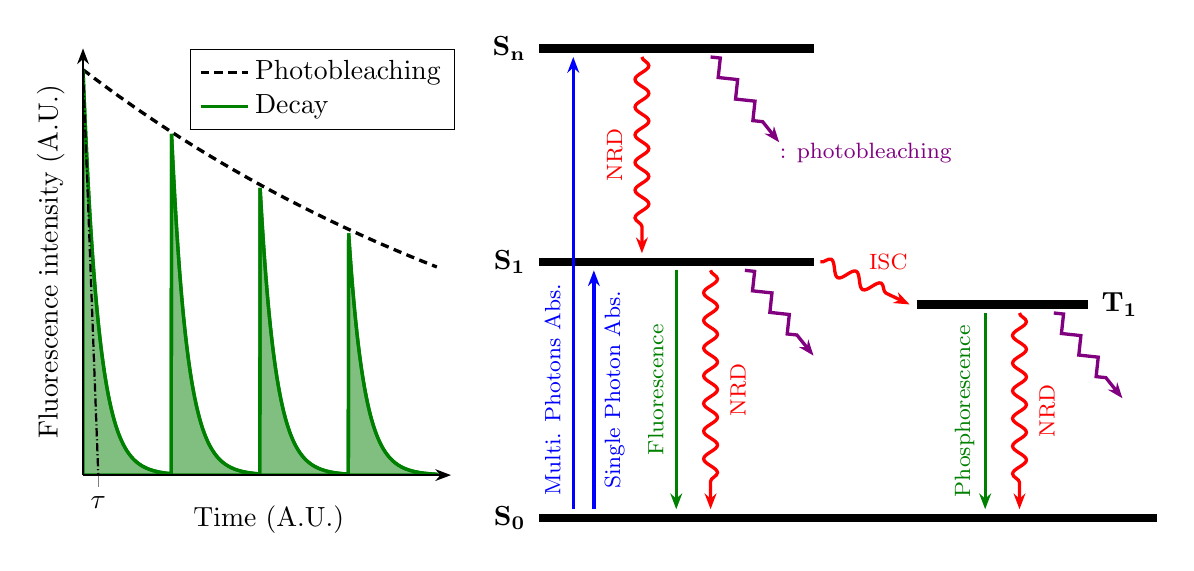
\begin{tikzpicture}	[
		declare function={
			func(\x)= (\x<2.5) * (0.95*(exp(-x/15))*exp(-\mtau*x))   +
			and(\x>=2.5, \x<5) * (0.95*(exp(-x/15))*exp(-\mtau*(x-2.5)))     +
			and(\x>=5,  \x<7.5) * (0.95*(exp(-x/15))*exp(-\mtau*(x-5))) +
			(\x>=7.5) * (0.95*(exp(-x/15))*exp(-\mtau*(x-7.5)));
		}
		]
		%\draw[draw=black] (-0.7,-1) rectangle ++(14.5cm,7cm);
		\begin{groupplot}[group style={group size=2 by 1, horizontal sep=0.2cm}]
		\nextgroupplot[
			width=6.3cm,
			legend cell align={left},
			tick align=outside,
			tick pos=left,
			xlabel={Time (A.U.)},
			xmin=0, xmax=10.5,
			xtick={0.95/\mtau},
			xticklabels={$\tau$},
			xlabel style={yshift=8pt},
			ylabel={Fluorescence intensity (A.U.)},
			ylabel style={yshift=-8pt},
			ymin=0, ymax=1,
			ytick style={color=black},
			yticklabels={},
			ytick style={draw=none},
			axis line style={draw=none},
			clip mode=individual,
			domain=0:7,
			samples=100,
			legend style={
				fill opacity=1,
				draw opacity=1,
				text opacity=1,
				at={(1.,1.)},
				anchor=north east,
				draw=black,
				xshift=+0.2pt,
				yshift=-0.2pt,
			},
			]
			
			% PBL
			\addplot[draw=black, densely dashed, no marks, \myline, domain=0:10., name path=risephospho] {0.95*(exp(-x/15))};
			\addlegendentry{Photobleaching}
			
			% pulses green
			\addplot[draw=Green, no marks, \myline, domain=0:10, name path=fluo1, samples=1000] {func(x)};
			\addlegendentry{Decay}
			
			% Filling in green
			\addplot[draw=none, no marks, \myline, domain=0:10, name path=mxaxis] {0};
			\addplot[Green!50, draw=Green, \myline] fill between[of=fluo1 and mxaxis];
			
			% Decay tau
			\addplot[draw=black, densely dashdotted, no marks, thick, domain=0:10.] {0.95 -\mtau*x};
			
			% xaxis
			\draw[-{Stealth[length=2mm]}, semithick] (0, 0) -- (10.4, 0); 
			
			% yaxis
			\draw[-{Stealth[length=2mm]}, semithick] (0,0) -- (0,1);
			
			%%%%%%%%%%%%%%%%%%%%%%%%%%%%%%%%%
			%%%%%%%%%%%%%%%%%%%%%%%%%%%%%%%%%
			\nextgroupplot[
			width=10.3cm,
			xmin=0, xmax=10,
			xtick style={draw=none},
			xticklabels={},
			ymin=0, ymax=10,
			ytick style={color=black},
			yticklabels={},
			ytick style={draw=none},
			axis line style={draw=none},
			clip mode=individual,
			]
			
			% Energy levels
			\draw[black, line width=3] (1,-1) node[left] {\textbf{S}$_\textbf{0}$} -- +(9,0);
			\draw[black, line width=3] (1,5) node[left] {\textbf{S}$_\textbf{1}$} -- +(4.,0);
			\draw[black, line width=3] (1,10) node[left] {\textbf{S}$_\textbf{n}$} -- +(4.,0);
			\draw[black, line width=3] (6.5,4) -- +(2.5,0) node[right] {\textbf{T}$_\textbf{1}$};
			
			% Absorbance
			\path [draw=blue, very thick, -{Stealth[length=2mm]}]
			(1.8,-0.8) -- (1.8,4.8);
			\node[anchor=center, rotate=90, blue] at
			(axis cs:2.1, 2) {\footnotesize{Single Photon Abs.}};
			\path [draw=blue, very thick, -{Stealth[length=2mm]}]
			(1.5,-0.8) -- (1.5,9.8);
			\node[anchor=center, rotate=90, blue] at
			(axis cs:1.2, 2) {\footnotesize{Multi. Photons Abs.}};
			
			% Sn NRD
			\path [draw=red,snake=snake, very thick, -{Stealth[length=2mm]}, line after snake=2mm]
			(2.5,9.8) -- (2.5,5.2);
			\node[anchor=center, rotate=90, red] at
			(axis cs:2.1, 7.5) {\footnotesize{NRD}};
			
			% Sn PBL
			\path [draw=violet,snake, very thick, -{Stealth[length=2mm]}, line after snake=2mm]
			(3.5,9.8) -- (4.5,7.8);
			\node[anchor=north west, inner sep=0, violet] at (axis cs:4.5, 7.8) {{\huge $\skull$}\raisebox{0.5em}{\footnotesize{: photobleaching}}};
			
			% Fluo
			\path [draw=Green, very thick, -{Stealth[length=2mm]}]
			(3,4.8) -- (3,-0.8);
			\node[anchor=center, rotate=90, Green] at
			(axis cs:2.7, 2) {\footnotesize{Fluorescence}};
			
			% S1 NRD
			\path [draw=red,snake=snake, very thick, -{Stealth[length=2mm]}, line after snake=2mm]
			(3.5,4.8) -- (3.5,-0.8);
			\node[anchor=center, rotate=90, red] at
			(axis cs:3.9, 2) {\footnotesize{NRD}};
			
			% S1 PBL
			\path [draw=violet,snake, very thick, -{Stealth[length=2mm]}, line after snake=2mm]
			(4.,4.8) -- (5.,2.8);
			\node[anchor=north west, inner sep=0, violet] at (axis cs:5, 2.8) {\huge $\skull$};
			
			% S1 T1 ISC
			\path [draw=red,snake=snake, very thick, -{Stealth[length=2mm]}, line after snake=2mm]
			(5.1,5) -- (6.4,4);
			\node[red, anchor=south west, inner sep=0] at (axis cs:5.8, 4.8) {\footnotesize{ISC}};
			
			% phospho
			\path [draw=Green, very thick, -{Stealth[length=2mm]}]
			(7.5,3.8) -- (7.5,-0.8);
			\node[anchor=center, rotate=90, Green] at
			(axis cs:7.2, 1.5) {\footnotesize{Phosphorescence}};
			
			% T1 NRD
			\path [draw=red,snake=snake, very thick, -{Stealth[length=2mm]}, line after snake=2mm]
			(8,3.8) -- (8.,-0.8);
			\node[anchor=center, rotate=90, red] at
			(axis cs:8.4, 1.5) {\footnotesize{NRD}};
			
			% T1 PBL
			\path [draw=violet,snake, very thick, -{Stealth[length=2mm]}, line after snake=2mm]
			(8.5,3.8) -- (9.5,1.8);
			\node[anchor=north west, inner sep=0, violet] at (axis cs:9.5, 1.8) {\huge $\skull$};
			
		\end{groupplot}
	\end{tikzpicture}
\end{document}